\documentclass[12pt, twoside]{article}
\usepackage[letterpaper, margin=1in, headsep=0.5in]{geometry}
\usepackage[english]{babel}
\usepackage[utf8]{inputenc}
\usepackage{amsmath}
\usepackage{amsfonts}
\usepackage{amssymb}
\usepackage{tikz}
%\usetikzlibrary{quotes, angles}

\usepackage{graphicx}
\usepackage{enumitem}
\usepackage{multicol}

\usepackage{fancyhdr}
\pagestyle{fancy}
\fancyhf{}
\renewcommand{\headrulewidth}{0pt} % disable the underline of the header

\usepackage{setspace}
%\linespread{1.75}

%\fancyhead[RE]{\thepage}
\fancyhead[R]{\thepage \\ Name: \hspace{3cm}}
\fancyhead[L]{BECA / Dr. Huson / 12.1 IB Math SL\\* 7 February 2019}

\begin{document}
\subsubsection*{Unit 5 Test: Integral Calculus}
 \begin{enumerate}

\subsubsection*{You may use a calculator on these problems \hfill [30 marks]}

\setstretch{2.0}

  \item Let $f(x)=x^3-4x^2-7$. Find $f'(x)$. \hfill [2]
  \item Let $f(x)=e^{3x-1}$. Find $f'(x)$. \hfill [2]
  \item Let $f(x)=x \sin x$. Find $f'(x)$. \hfill [2]
  \item Let $f(x)=\sqrt{x} + \ln x$. Find $f'(x)$. \hfill [2]

  \item Find $\int x^3 \,\mathrm{d}x$. \hfill [2]
  \item Find $\int \sin x \,\mathrm{d}x$. \hfill [2]
  \item Find $\int e^{3x} \,\mathrm{d}x$. \hfill [2]
  \item Find $\int (2x+4)(x^2+4x)^3 \,\mathrm{d}x$. \hfill [2]

  \item Find $\int_0^2 x^2 e^{-x} \,\mathrm{d}x$. \hfill [4]
  \item Find $\int_0^3 x - e^{0.5x}+3 \,\mathrm{d}x$. \hfill [4] \vspace{1.0cm}

  \setstretch{1.0}

   \item Let $f(x)=xe^{-x}$ and $g(x)=-3f(x)+1$. \hfill [6 marks]\\
   The graphs of $f$ and $g$ intersect at $x=p$ and $x=q$, where $p<q$.
   \begin{enumerate}
     \item Find the values of $p$ and $q$. \hfill [3] \vspace{1.5cm}
     \item Hence, find the area of the region enclosed by the graphs of $f$ and $g$. \hfill [3]
   \end{enumerate}

\newpage
\subsubsection*{No Calculator section \hfill [38 marks]}

  \item Let $f(x)=3x^2-x$. The graph of $f$ is shown in the following diagram. \hfill [6 marks]
    \begin{center}
      \begin{tikzpicture}[xscale=1.5,yscale=0.28]
        \draw [thick, ->] (0,0) -- (4,0) node [below] {$x$};
        \draw [thick, ->] (0,-3) -- (0,12) node [left] {$y$};
        \draw[thick, domain=0:2.1] plot[samples=100](\x, {3*(\x)^2 - (\x)});
        \draw[thick] (1, -.5)node[below]{$1$} --(1,2);
        \draw[thick] (2, -.5)node[below]{$2$} --(2,10);
      \end{tikzpicture}
    \end{center}
    \begin{enumerate}
      \item Find $f'(x)$. \hfill [2]  \vspace{1.5cm}
      \item Find the area of the region enclosed by the graph of $f$, the $x$-axis and the lines $x = 1$ and $x = 2$. \hfill [4]
    \end{enumerate} \vspace{1.5cm}

    \item Consider a function $f(x)$ such that $\int_1^6 f(x) \,\mathrm{d}x
=8$. \hfill [6 marks]
    \begin{enumerate}
      \item Find $\int_1^6 2f(x) \,\mathrm{d}x$. \hfill [2] \vspace{1.5cm}
      \item Find $\int_1^6 (f(x)+2) \,\mathrm{d}x$. \hfill [4]
    \end{enumerate} \vspace{1.5cm}

    \item 14M.1.sl.TZ2.5 \hfill [6 marks]\\
    The graph of a function $h$ passes through the point $(\frac{\pi}{12},5)$.\\
    Given that $h'(x)=4 \cos 2x$, find $h(x)$. \hfill [6]



\newpage

    \item 18M.2.sl.TZ1.4 \hfill [7 marks]\\
    Let  $g(x)=-(x-1)^2+5$.
    \begin{enumerate}
      \item Write down the coordinates of the vertex of the graph of $g$. \hfill [1]
      \item Let $f(x)=x^2$. The following diagram shows part of the graph of $f$.
        \begin{center}
        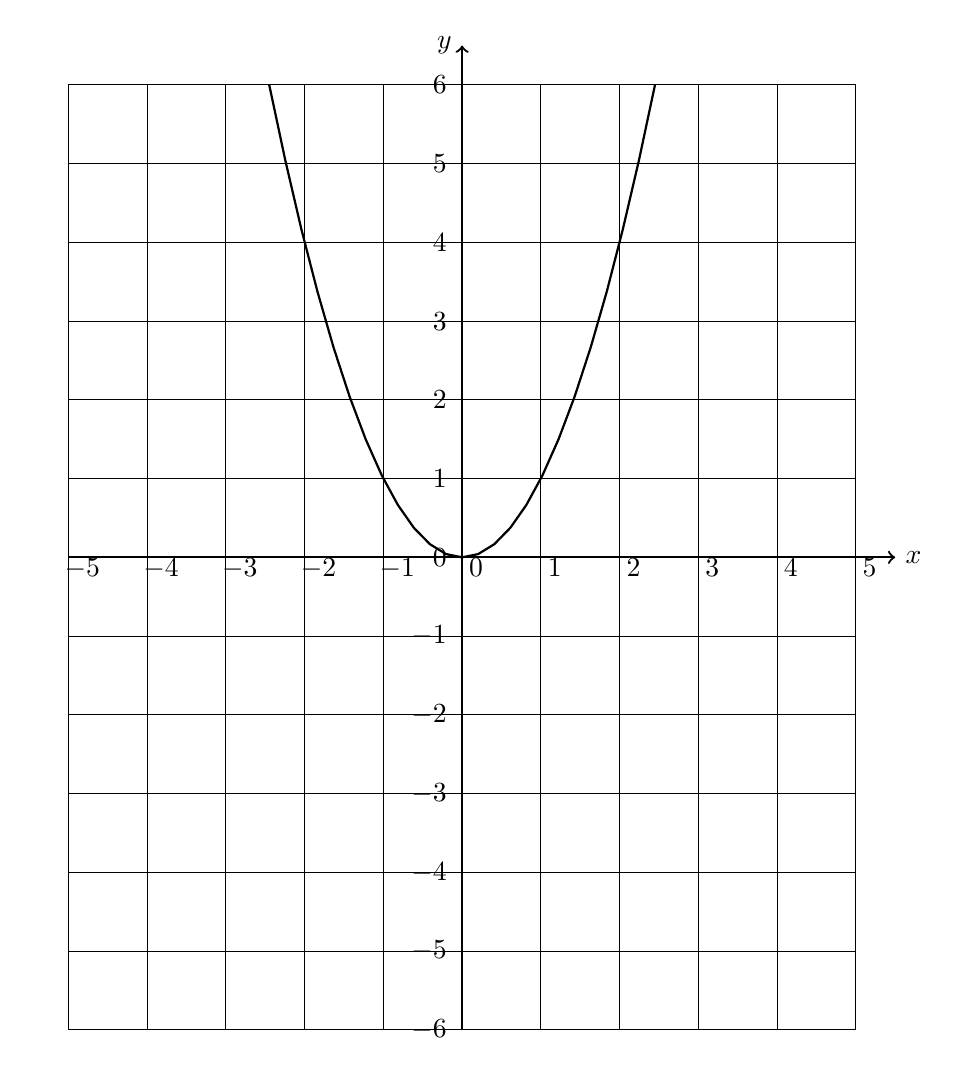
\begin{tikzpicture}%[scale=0.7]
          \draw [black, xstep=1.0cm, ystep=1.0cm] (-5,-6) grid (5,6);
          %\draw [gray, very thin, xstep=0.2cm, ystep=0.2cm] (0,-5) grid (10,5);
          \foreach \x in {-5,...,5}
          \draw[shift={(\x,0)},color=black] (0pt,-1pt) -- (0pt,3pt) node[below]  {$\quad \x$};
          \foreach \y in {-6,...,6}
          \draw[shift={(0,\y)},color=black] (2pt,0pt) -- (-2pt,0pt) node[left]  {$\y$};
          \draw [thick, ->] (-5,0) -- (5.5,0) node [right] {$x$};
          \draw [thick, ->] (0,-6) -- (0,6.5) node [left] {$y$};
          \draw [thick,domain=-(sqrt(6)):(sqrt(6))] plot(\x,{(\x)^2});
        \end{tikzpicture}
        \end{center}
      The graph of $g$ intersects the graph of $f$ at $x=-1$ and $x=2$.\\
      On the grid above, sketch the graph of $g$ for $-2 \leq x \leq 4$. \hfill [3]
      \item Find the area of the region enclosed by the graphs of $f$ and $g$. \hfill [3]
    \end{enumerate} \vspace{1.5cm}

    \item A function $f(x)$ has derivative $f'(x) = 3x^2 + 18x$. The graph of $f$ has an $x$-intercept at $x = -1$. \hfill [13 marks]
    \begin{enumerate}
      \item Find $f(x)$. \hfill [6]
      \item The graph of $f$ has a point of inflexion at $x = p$. Find $p$. \hfill [4]
      \item Find the values of $x$ for which the graph of $f$ is concave-down. \hfill [3]
    \end{enumerate}


\end{enumerate}
\end{document}

  \newpage

    \item 17M.1.sl.TZ2.5 \hfill [6 marks]\\
    Let $\displaystyle f'(x)=\frac{3x^2}{(x^3+1)^5}$. Given that $f(0)=1$, find $f(x)$. \hfill [6]

    \item 17M.1.sl.TZ1.5a \hfill [7 marks]
    \begin{enumerate}
      \item Find $\int x e^{x^2-1} \,\mathrm{d}x$. \hfill [4]
      \item Find $f(x)$, given that $f'(x) = x e^{x^2-1}$ and $f(-1)=3$ \hfill [3]
    \end{enumerate}

%\newpage
\subsubsection*{Spicy: Extended response}

  \item 16M.1.sl.TZ1.10 \hfill [15 marks]\\
  Let $f(x)=\sqrt{4x+5}$, for $x \geq -1.25$.
  \begin{enumerate}
    \item Find $f'(1)$. \hfill [4]
    \item Consider another function $g$. Let $R$ be a point on the graph of $g$. The $x$-coordinate of $R$ is 1. The equation of the tangent to the graph at $R$ is  $y=3x+6$.\\
    Write down $g'(1)$. \hfill [2]
    \item Find $g(1)$. \hfill [2]
    \item Let $h(x)=f(x) \times g(x)$. Find the equation of the tangent to the graph of $h$ at the point where $x=1$. \hfill [7]
  \end{enumerate}

\newpage

    \item (\#19) 17N.1.sl.TZ0.8 \hfill [16 marks]\\
    Let $f(x)= x^2-x$, for $x \in \mathbb{R}$. The following diagram shows part of the graph of $f$.
      \begin{center}
        \begin{tikzpicture}[xscale=0.75, yscale=0.5]
          \draw [thick, ->] (-3,0) -- (4,0) node [below] {$x$};
          \draw [thick, ->] (0,-2) -- (0,10) node [left] {$y$};
          \draw[thick, domain=-2.5:3.5] plot[samples=100](\x, {(\x)^2 - \x});
          \node at (1,0) {\textbullet};
          \node at (1,0)[below] {\textbf{P}};
          \node at (2,6) {$f$};
          \node at (4,8)[right] {\textbf{diagram not to scale}};
        \end{tikzpicture}
      \end{center}
      The graph of $f$ crosses the $x$-axis at the origin and at the point $P(1,0)$.
      \begin{enumerate}
        \item Show that $f'(1)=1$. \hfill [3]
        \item The line $L$ is the normal to the graph of $f$ at $P$.\\
        Find the equation of $L$ in the form $y=ax+b$. \hfill [3]
        \item The line $L$ intersects the graph of $f$ at another point $Q$, as shown in the following diagram.
          \begin{center}
            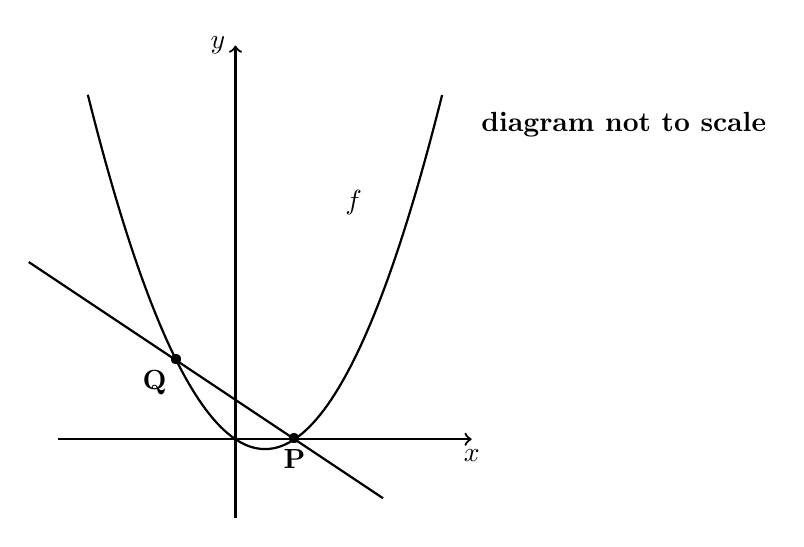
\begin{tikzpicture}[xscale=0.75, yscale=0.5]
              \draw [thick, ->] (-3,0) -- (4,0) node [below] {$x$};
              \draw [thick, ->] (0,-2) -- (0,10) node [left] {$y$};
              \draw[thick, domain=-2.5:3.5] plot[samples=100](\x, {(\x)^2 - \x});
              \draw[thick, domain=-3.5:2.5] plot[samples=100](\x, {(-\x+1});
              \node at (1,0) {\textbullet};
              \node at (1,0)[below] {\textbf{P}};
              \node at (2,6) {$f$};
              \node at (4,8)[right] {\textbf{diagram not to scale}};
              \node at (-1,2) {\textbullet};
              \node at (-1,2)[below left] {\textbf{Q}};
            \end{tikzpicture}
          \end{center}
          Find the $x$-coordinate of $Q$.\hfill [4]
          \item Find the area of the region enclosed by the graph of $f$ and the line $L$.  \hfill [6]
      \end{enumerate}

\newpage

    \item (\#23) 17M.1.sl.TZ2.10 \hfill [17 marks]\\
    Let $f(x)= x^2$. The following diagram shows part of the graph of $f$.
        \begin{center}
          \begin{tikzpicture}[xscale=4, yscale=3]
            \draw [thick, ->] (-1.5,0) -- (1,0) node [below] {$x$};
            \draw [thick, ->] (0,-.5) -- (0,1.5) node [left] {$y$};
            \draw [thick, domain=-1.2:0.75] plot[samples=100](\x, {(\x)^2});
            \draw [thick] (-1.25,1.5)node[left]{$L$}
              --(-0.5,0)node[below left]{\textbf{B}} --(-0.3,-0.45);
            \node at (-0.5,0) {\textbullet};
            \node at (-1,1) {\textbullet};
            \node at (-1,1)[right] {\textbf{A}$(-k,k^2)$};
            \node at (-1,0) {\textbullet};
            \node at (-1,0)[below] {\textbf{C}$(-k,0)$};
            \node at (0.55,0.5) {$f$};
            \node at (1,1)[right] {\textbf{diagram not to scale}};
          \end{tikzpicture}
        \end{center}
      The line $L$ is the tangent to the graph of $f$ at the point $A(-k,k^2)$, and intersects the $x$-axis at point $B$. The point $C$ is $(-k,0)$.
      \begin{enumerate}
        \item Write down $f'(x)$. \hfill [1]
        \item Find the gradient of $L$. \hfill [2]
        \item Show that the $x$-coordinate of $B$ is $-\frac{k}{2}$. \hfill [5]
        \item Find the area of triangle $ABC$, giving your answer in terms of $k$. \hfill [2]
        \item The region $R$ is enclosed by $L$, the graph of $f$, and the $x$-axis. This is shown in the following diagram.
          \begin{center}
            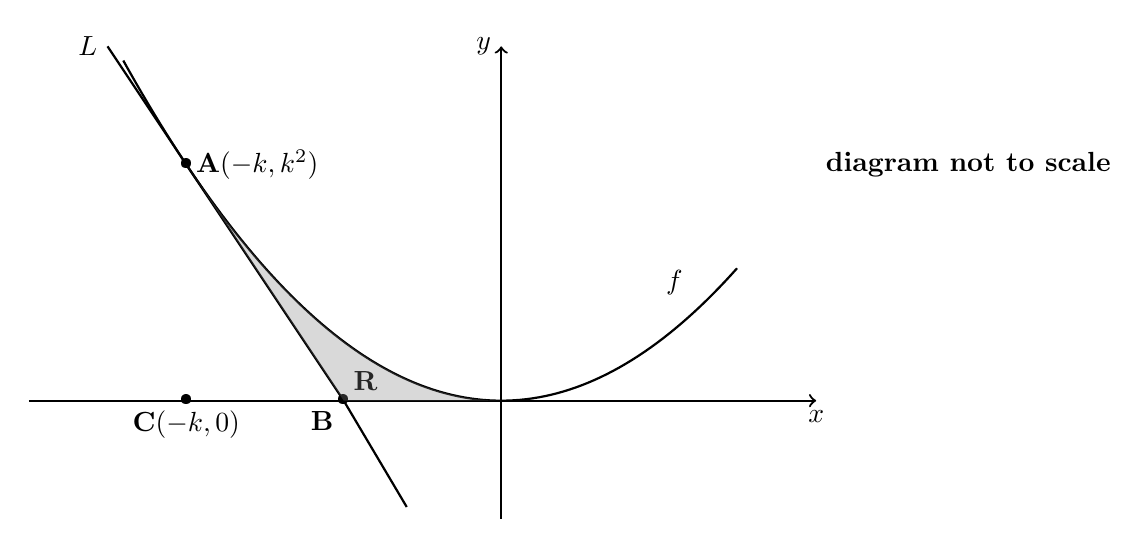
\begin{tikzpicture}[xscale=4, yscale=3]
              \draw [thick, ->] (-1.5,0) -- (1,0) node [below] {$x$};
              \draw [thick, ->] (0,-.5) -- (0,1.5) node [left] {$y$};
              \draw [thick, domain=-1.2:0.75] plot[samples=100](\x, {(\x)^2});
              \draw [thick] (-1.25,1.5)node[left]{$L$}
                --(-0.5,0)node[below left]{\textbf{B}} --(-0.3,-0.45);
              \node at (-0.5,0) {\textbullet};
              \node at (-0.5,0) [above right] {$\mathbf{R}$};
              \node at (-1,1) {\textbullet};
              \node at (-1,1)[right] {\textbf{A}$(-k,k^2)$};
              \node at (-1,0) {\textbullet};
              \node at (-1,0)[below] {\textbf{C}$(-k,0)$};
              \node at (0.55,0.5) {$f$};
              \node at (1,1)[right] {\textbf{diagram not to scale}};
              \fill[gray,opacity=.3] (-0.5,0) -- plot[domain=-1:0](\x,{(\x)^2});
            \end{tikzpicture}
          \end{center}
        Given that the area of triangle $ABC$ is $p$ times the area of $R$, find the value of $p$.  \hfill [7]
      \end{enumerate}


\end{enumerate}
\end{document}
